
\section{Results}
\label{sec:results}

\begin{figure}

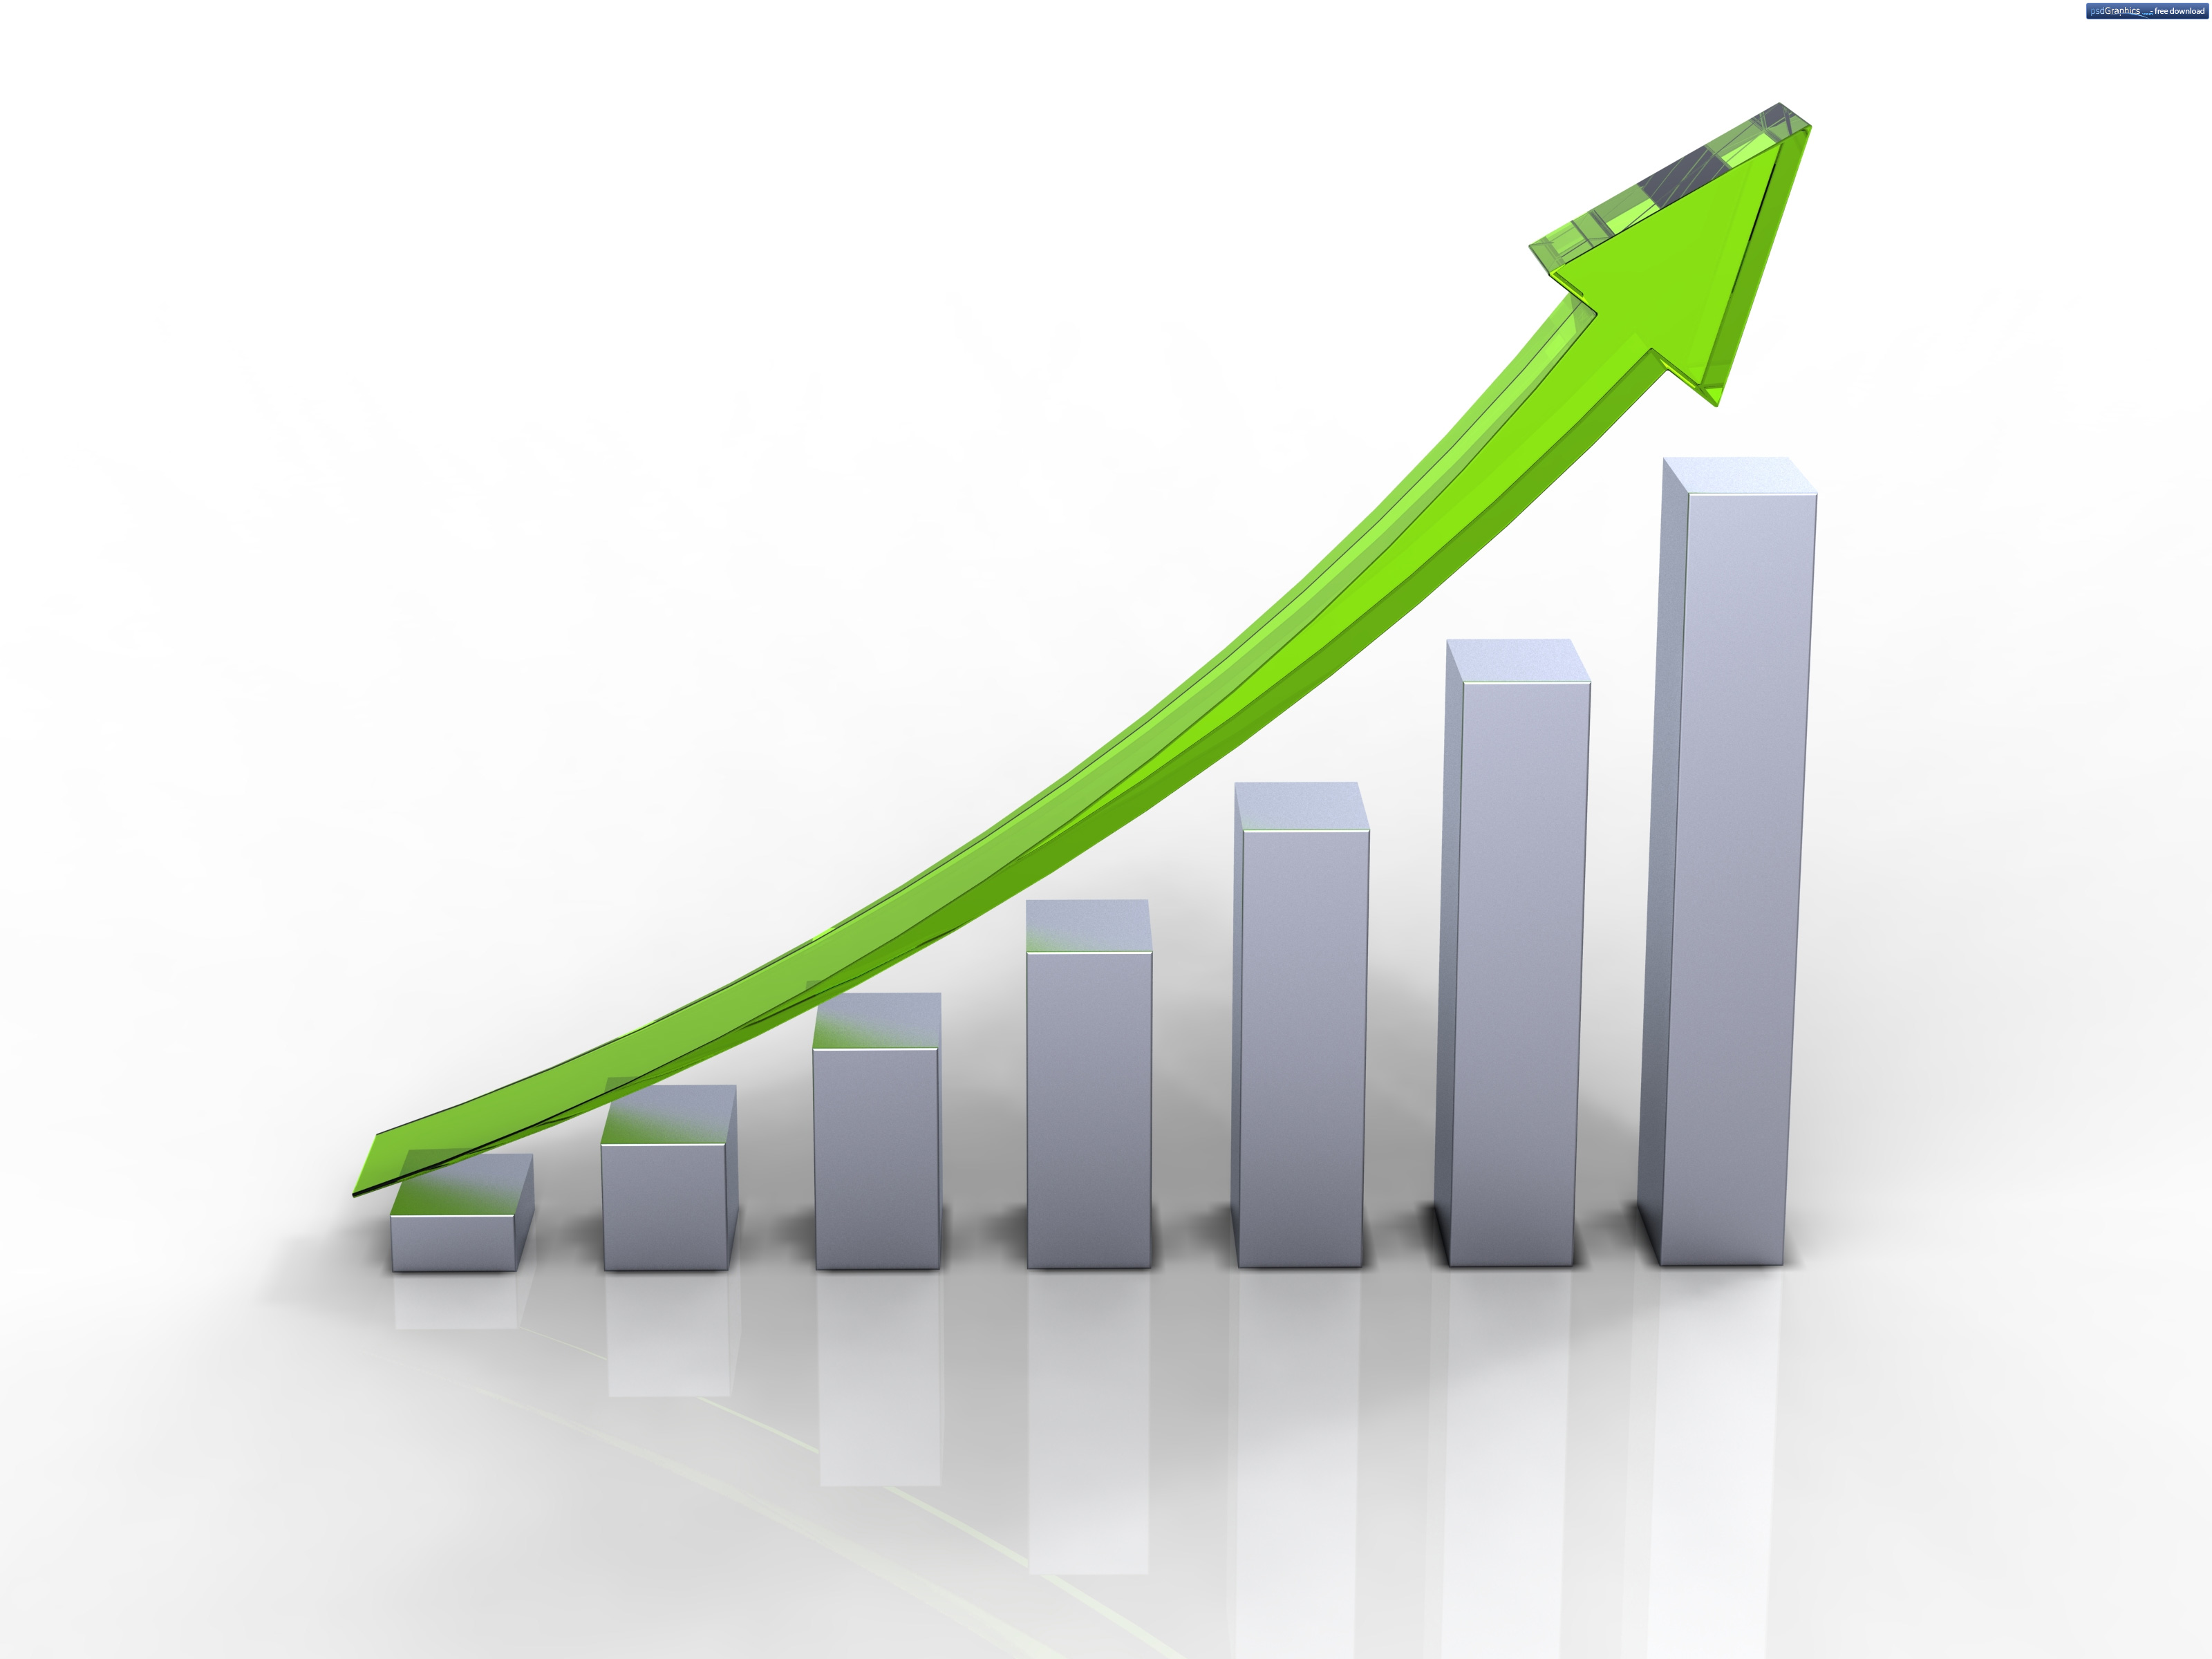
\includegraphics[keepaspectratio, width=0.35\textheight]
{./img/graph.jpg}
\caption{Sample of a graph}
\label{fig:graph}
\end{figure}

<<<<<<< HEAD
Lorem ipsum dolor sit amet, consectetur adipiscing elit. Sed eget purus in mi fringilla faucibus ut sit amet enim. Integer ac aliquam lacus. Sed semper luctus leo, a porttitor ligula. Praesent elementum placerat mi. Maecenas suscipit convallis justo, eget aliquam neque blandit vitae. Sed tincidunt dui nec metus sagittis, a semper nibh luctus. Pellentesque felis tortor, interdum sed congue sed, bibendum vitae eros. Suspendisse fringilla bibendum pretium. Vivamus at eros ac urna consectetur auctor.
=======
\begin{table}
\centering
\begin{tabular}{ | l | c | }
	\hline
	Vertices & 1,000,000 \\ \hline
	Edges & 8,700,950 \\ \hline
	Partitions & 8 \\ \hline
	\# client requests & 100,000 \\ \hline
	\# clients & 8 \\ \hline
	\# threads/client & 10 \\ \hline
\end{tabular}
\caption{Configuration used for our evaluations}
\label{tbl:graphconfig}
\end{table}

Lorem ipsum dolor sit amet, consectetur adipiscing elit. Sed eget purus in mi fringilla faucibus ut sit amet enim. Integer ac aliquam lacus. Sed semper luctus leo, a porttitor ligula. Praesent elementum placerat mi. Maecenas suscipit convallis justo, eget aliquam neque blandit vitae. Sed tincidunt dui nec metus sagittis, a semper nibh luctus. Pellentesque felis tortor, interdum sed congue sed, bibendum vitae eros. Suspendisse fringilla bibendum pretium. Vivamus at eros ac urna consectetur auctor.
>>>>>>> a21da72e60514db4c40d0fe0ffb3a6df2772a64e
